\documentclass[10pt]{article}
\newcommand{\HRule}{\rule{\linewidth}{0.5mm}}
\parindent 0pt
\parskip 10pt
\usepackage{anysize}
\usepackage{graphicx}
\usepackage{epsfig}
\usepackage{float}
%\usepackage{cite}
\usepackage{natbib}
\usepackage{setspace}
\marginsize{3.5cm}{3.5cm}{1cm}{1cm}
\onehalfspacing
\usepackage{caption}
\usepackage{subcaption}
\usepackage{amsmath,hyperref}

\usepackage{xcolor}
\hypersetup{
    colorlinks,
    linkcolor={red!50!black},
    citecolor={blue!50!black},
    urlcolor={blue!80!black}
}

%\textwidth 15cm
%\textheight 24cm
%\onehalfspacing
\begin{document}

\title{Football Exercise}

\author{David Starkey}

\maketitle






Please see the documentation of my answers to the football exercise below. I will begin with a brief sumary of the data set and the python modules used to ingest it before proceeding on to answer each of the 9 questions in turn. My source code can be found in \verb|main_code.py| and predictions in \verb|predictions.csv|.  

The training data was ingested using the pandas module in python (see lines 15 to 21 of the attached source code). This is a fast effective way to load data, requires only a few lines of code to prepare the data ready for all the necessary visualisation and algebraic manipulation that follows.



\section{1) Expected Goals of Home and Away Team Individually}
\label{sec_1}

The training data contains the expected total number of goals $T = E(H+A)$ and the expected supremacy $S = E(H-A)$. The individual expected home and away goals is then given by 

\begin{equation}
\label{eq_h_expected}
E(H) = \frac{E(H+A) + E(H-A)}{2} = \frac{T+S}{2}
\end{equation}
\noindent and
\begin{equation}
\label{eq_a_expected}
E(A) = \frac{E(H+A) - E(H-A)}{2} = \frac{T-S}{2}
\end{equation}
\noindent respectively.





\section{2) Poisson Distribution}
\label{sec_poisson}

I treat the number of the home and away scores for the full game as a Poison distribution. This takes the form

\begin{equation}
P(n|\mu) = e^{-\mu}\frac{\mu^n}{n!},
\end{equation}

\noindent where $n$ is the number of goals in a match with an expected number of goals $\mu$ (see Figure \ref{fig_poison}).

The required assumptions of this distribution are ideal for modelling goals in a football match. These are namely:

\begin{itemize}
\item The outcomes are discrete (1, 2, 4 not 1.5, 1.2 etc). 

\item Only positive outcomes are allowed (no negative goals).

\item The goal rate in a given match is constant and unaffected by the number of goals that came before it within a given match (events within a match are independent)\footnote{This will be important later when the first and second halves are modelled separately}.



\end{itemize}





\begin{figure}
\begin{center}
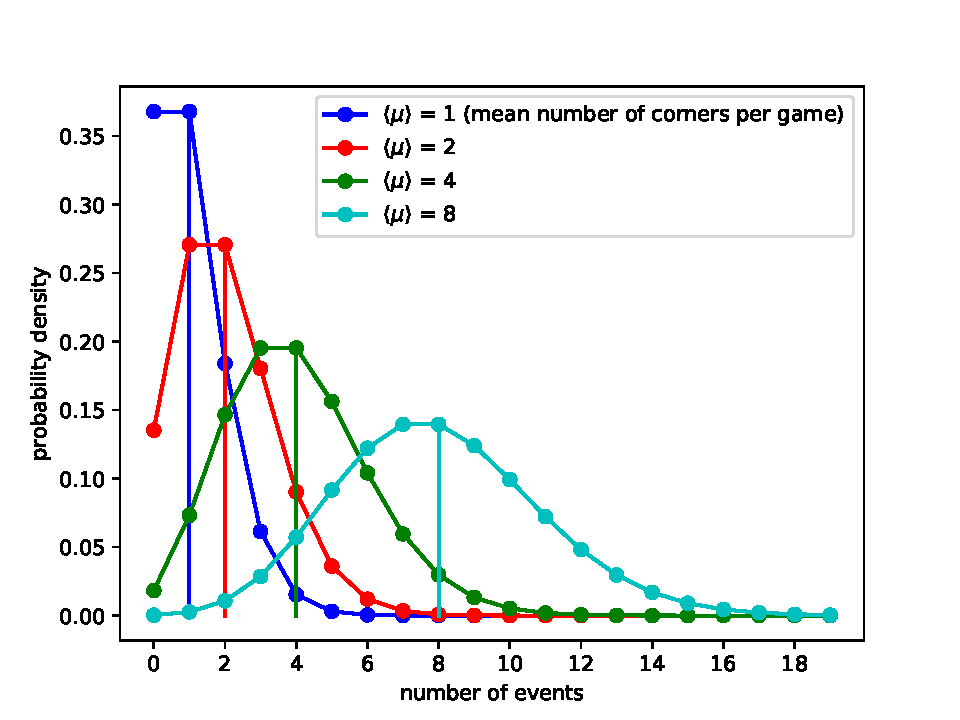
\includegraphics[scale=1.0,angle=0,trim=0cm 0cm 0cm 0cm]{fig_poison.pdf}
\caption{Example Poisson distributions for a selection of expected $\mu$ values. Vertical lines and the legend indicate the value of $\mu$.}
\label{fig_poison}
\end{center}
\end{figure} 




\section{3) Poisson Distribution Appplied to specific game}

The attached code in \verb|main_code.py| documents how this is achieved for question 3. An example game is given with expected home and away team scores 1.6 and 0.9 respectively. The outcome is modelled as joint Poisson distributions for the home $P(h|E(h))$ and away $P(a|E(a))$ scores respectively such that the joint probability of a particular home away score $P(h,a|E(h),E(a))$ is given by

\begin{equation}
\label{eq_joint}
P(h,a|E(h),E(a)) = P(h|E(h)) P(a|E(a))
\end{equation} 
\noindent. All possible combinations of $h$ and $a$ are input into Equation \ref{eq_joint} considering goals 0...9. The probability of score 0,0 is found to be 0.082.


\section{4) Probability of winning the game}
\label{sec_win}
To calculate the win probability, all probabilities $P(h,a|E(h),E(a))$ are summed together for which $h>a$. This is found to be 0.538.





\begin{figure}
\begin{center}
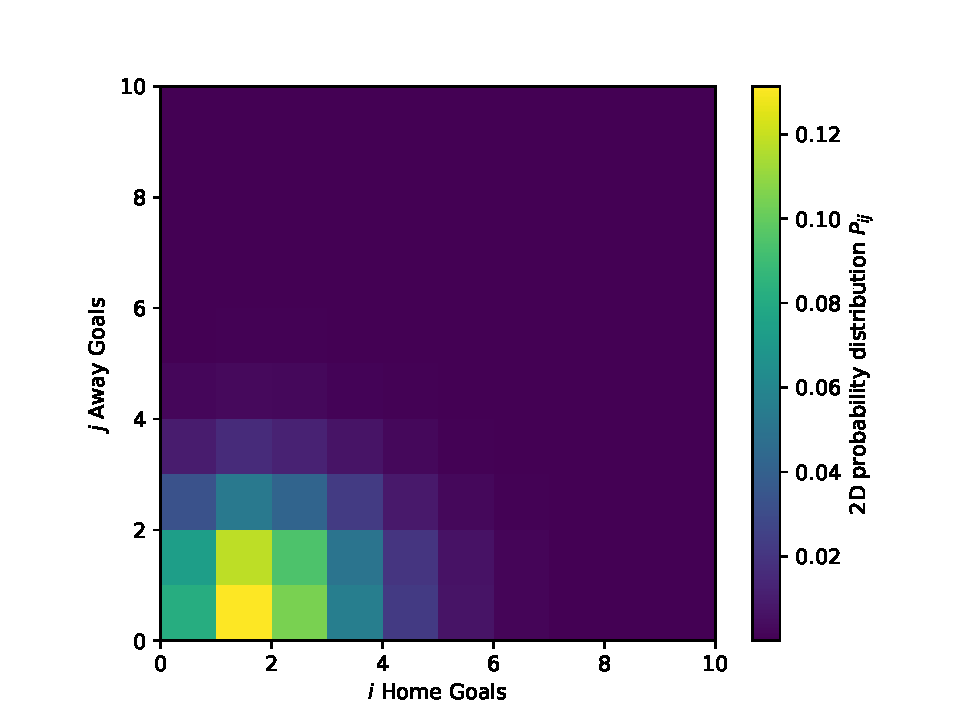
\includegraphics[scale=1.0,angle=0,trim=0cm 0cm 0cm 0cm]{fig_eg_posterior.pdf}
\caption{Example posterior probability distributions for the example game in Question 3. The 2D posterior probability distributions are computed using Equation \ref{eq_joint}. }
\label{fig_posterior_eg}
\end{center}
\end{figure} 







\section{5) How can we construct expected goals at half time for each team using the data provided?}

Returning to the assumptions of the Poisson distribution. We strictly require events to be independent. That is that a goal early in the match should not change the probability of goals later in the match. Also we require events to be regular. Therefore the expectation value of the number of goals in the second half $E(2)$ should equal that in the first half (at half time) $E(1)$ such that $E(1) = E(2)$. The totoal expectation value $T$ (see also Equations \ref{eq_h_expected} and \ref{eq_a_expected}) should be given by

\begin{equation}
\label{eq_e12_should}
T = E(1) + E(2) = 2E(1),
\end{equation}
\noindent where the expected goals at half time $E(1)$ is then just $T/2$.

We can test this by computing the histogram of actual scores in the first and second half of the matches in the training data. Figure \ref{fig_hist12} shows that there is a slight bias toward more goals being scored in the second than first half of a match. The expected values of the two distributions $E(1)$ and $E(2)$ are related by 

\begin{equation}
\label{eq_x12}
E(2) = XE(1),
\end{equation}
\noindent where (from Figure \ref{fig_hist12}) $X = 1.27$.

Given the expected value of the scores at half time $T$, the expected score at half time $E(1)$ can be calculate using 

\begin{equation}
\label{eq_ex_half_x_halfway}
T = E(1) + E(2) = E(1) \left(1 + X \right),
\end{equation}

\noindent on rearranging this yields the result for $E(1)$ where

\begin{equation}
\label{eq_ex_half_x}
E(1) =\frac{T}{ \left(1 + X \right)}.
\end{equation}

\noindent For completeness, $E(2)$ is given by
\begin{equation}
\label{eq_ex_half_x_e2}
E(1) =\frac{T}{ \left(1 + \left( 1/X\right) \right)}.
\end{equation}





\begin{figure}
\begin{center}
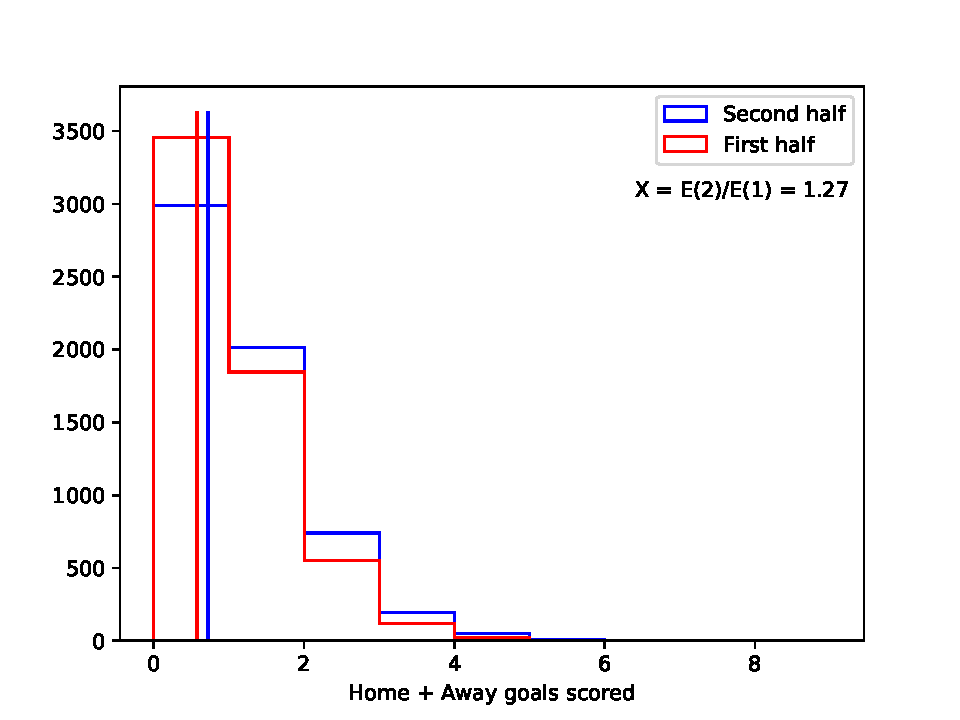
\includegraphics[scale=1.0,angle=0,trim=0cm 0cm 0cm 0cm]{fig_1st_2nd_comp_tot.pdf}
\caption{Histogram showing the distribution of goals in the first and second half respectively. Vertical lines show the mean of the distribution and $X = E(2)/E(1)$ is the factor by which the expected number of goals in the second half exceeds that in the first half.}
\label{fig_hist12}
\end{center}
\end{figure} 






\section{6) Is the number of goals at full time independent of the number of goals scored at half time}

Equation \ref{eq_ex_half_x_halfway} shows that the number of goals scored at full time does indeed depend on the number of goals scored at half time. It should be twice $E(1)$ given that we would prefer events to be independent and evenly sample when using a Poisson distribution, but here I have introduced the small correction $X$ to allow for the higher expected scores in the second half. 




\section{7) Probability of home team leading 1-0 at half time then winning 2-1 at full time}
The expected goals of the home and away teams after the first half are now given by 
\begin{equation}
\label{eq_eh1}
E(h_1) =\frac{E(h)}{ \left(1 + X \right)},
\end{equation}
\noindent and
\begin{equation}
\label{eq_ea1}
E(a_1) =\frac{E(a)}{ \left(1 + X \right)},
\end{equation}

\noindent where $E(h)$ and $E(a)$ were derived in Question 1 (Equations \ref{eq_h_expected} and \ref{eq_a_expected}). I now model the first and second halves of each game separately assuming a joint Poisson distribution as with Question 3 (Equation \ref{eq_joint}). The probability of scores at half time (denoted by subscript 1) is explicitly given by

\begin{equation}
\label{eq_joint_1st}
P(h_1,a_1|E_1(h_1),E_1(a_1)) = P(h_1|E_1(h_1)) P(a_1|E_1(a_1)).
\end{equation}

\noindent The probability of scores in the second half is then given by
\begin{equation}
\label{eq_joint_2st}
P(h_2,a_2|E_2(h_2),E_2(a_2)) = P(h_2|E_2(h_2)) P(a_2|E_2(a_2)),
\end{equation}
\noindent and the probability of a certain score in the first half and certain score in the second half is given by
\begin{equation}
\label{eq_joint_both}
P(h_1,a_1,h_2,a_2|E_1(h_1),E_1(a_1),E_2(h_2),E_2(a_2)) = P(h_1,a_1|E_1(h_1),E_1(a_1)) P(h_2,a_2|E_2(h_2),E_2(a_2)).
\end{equation}


\noindent The probability of the home team leading 1-0 at half time then winning 2-1 at full time assuming home and away team expected full time scores of $E(H) =  1.6$ and $E(A) = 0.9$ is then $P(1,0,1-1,1-0|E_1(h_1),E_1(a_1),E_2(h_2),E_2(a_2)) = 0.037$ where the expectation values $E_1(h_1),E_1(a_1),E_2(h_2),E_2(a_2)$ are calculated from $X$ using Equation\ref{eq_ex_half_x} 




\section{8) Probability of joint draw at half time and away team winning at full time}
\label{sec_8}

I now use the same principle as in Section \ref{sec_win} to calculate the probability of the double score of draw at half time and win at full time. The full combination of probabilities for all possible scores (up to 9 goals) is stored in arrays calculated using Equations \ref{eq_joint_1st} to \ref{eq_joint_both}. The trick now is to sum the probabilities of all scores in the first half that count as a draw (e.g 00, 11, 22, 33 etc). This is done in the attached code and the summed probabilities of a draw in the first half is 0.085.


\section{9) For all games in test data set. Predict all combinations of double scores hh,hd,ha,dh,dd,da,ah,ad,aa}
\label{sec_9}

This will use the formulation set out in Equation \ref{eq_joint_both}, using the X value of 1.27 calculated from the training set (Figure \ref{fig_hist12}). Equations \ref{eq_h_expected} and \ref{eq_a_expected} are used to compute the expected full-time home and away scores from the supremacy and expected full time total scores provided in the test data. Given $E(h)$ and $E(a)$, Equations \ref{eq_ex_half_x} and \ref{eq_ex_half_x_e2} are used to compute the expected 1st and 2nd half scores for the home and away teams. Since we consider scores 0 to 9, there are 10 x 10 x 10 x 10 possible outcomes to consider for each game relating the to possible home and away scores in the first and second half. This is arranged in an array with a row per game in the test set and columns that are given by \verb|h1,a1,h2,a2,P(h_1,a_1,h_2,a_2)|. From this array elements where $h1>a1$ constitute a home win in the first half. Elements where $h1+h2>a1+a2$ correspond to a home win at full time. Python searches through this array summing appropriate probabilities to construct the output \verb|predictions.csv| file with the requested information.






\end{document}



